Atom vodíku je asi nejsložitější soustava, kterou jsme schopni analyticky přesně vyřešit. Tato situace je pro chemika pochopitelně málo uspokojivá. Pomocí kvantové teorie bychom chtěli zkoumat vlastnosti atomů a molekul, ve kterých se pohybuje mnoho elektronů! Příslušné Schr\"odingerovy rovnice jsou ale příliš komplikované, takže nejsme schopni naleznout řešení analytické a bohužel ani řešení numericky přesné. Nezbývá nám proto než se vydat do kalných vod přibližných metod. Řešení Schr\"odingerovy rovnice pro atom vodíku nám nicméně poskytne dobrý základ, ze kterého je možné se odrazit k~přibližnému řešení problému více-elektronových atomů. Základní postupy si můžeme ukázat již na \uv{nejjednodušším složitém atomu}, atomu helia.  

\subsection{Atom helia}
V~atomu helia na sebe působí tři částice, jádro helia s~protonovým (resp. nábojovým) číslem $Z = 2$ a dva elektrony. Nebude nám tudíž zatěžko napsat pro helium hamiltonián 

\begin{equation}
\hat{H} = - \frac{\hbar^2}{2 m_e} \left( \Delta e_1 + \Delta e_2 \right) - \frac{1}{4 \pi \epsilon_0} \left(\frac{2e^2}{r_1} + \frac{2e^2}{r_2} \right) + \frac{1}{4 \pi \epsilon_0} \frac{e^2}{r_{12}},
\label{rov:VE-1}
\end{equation}


\noindent kde hamiltonián zapisujeme v~souřadnicové soustavě umístěné do jádra helia.
\begin{equation}
\Delta_{e_1} \equiv \frac{\partial^2}{\partial x_{e1}^2} + \frac{\partial^2}{\partial y_{e1}^2}+\frac{\partial^2}{\partial z_{e1}^2} \nonumber
\end{equation}
je Laplaceův operátor prvního elektronu popisující kinetickou energii prvního elektronu,
\begin{equation}
\Delta_{e_2} \equiv \frac{\partial^2}{\partial x_{e2}^2} + \frac{\partial^2}{\partial y_{e2}^2}+\frac{\partial^2}{\partial z_{e2}^2} \nonumber
\end{equation}
je Laplaceův operátor příslušející druhému elektronu, $r_1$ je vzdálenost mezi jádrem helia a~prvním elektronem, $r_2$ je vzdálenost mezi jádrem helia a druhým elektronem,a $r_{12}$ je vzdálenost mezi oběma elektrony. Schr\"odingerova rovnice je v~tomto případě parciální diferenciální rovnicí druhého řádu, jejímž řešením je (vlnová) funkce šesti proměnných, kupříkladu kartézských souřadnic obou elektronů $x_1$, $y_1$, $z_1$, $x_2$, $y_2$ a $z_2$ nebo sférických souřadnic těchto elektronů $r_1$, $\theta_1$, $\phi_1$, $r_2$, $\theta_2$, $\phi_2$. Bohužel, ani v~jedné sadě souřadnice se nám nepodaří hamiltonián separovat, nemůžeme jej napsat jakou součet členu závisejících na souřadnicích pouze jednoho elektronu a členu závisejícího pouze na souřadnicích elektronu druhého. Hamiltonián můžeme zapsat následujícím způsobem

\begin{equation}
\hat{H} = \hat{H}_1 + \hat{H}_2 + \hat{H}_{12},
\label{rov:VE-2}
\end{equation}

\noindent kde hamiltonián 

\begin{equation}
\hat{H}_1 = - \frac{\hbar^2}{2 m_e} \Delta_1 - \frac{1}{4 \pi \epsilon_0} \frac{2 e^2}{r_1}
\label{rov:VE-3}
\end{equation} 

\noindent působí toliko na souřadnice prvního elektronu a hamiltonián 

\begin{equation}
\hat{H}_2 = - \frac{\hbar^2}{2 m_e} \Delta_2 - \frac{1}{4 \pi \epsilon_0} \frac{2 e^2}{r_2}
\label{rov:VE-4}
\end{equation}

\noindent pouze na souřadnice elektronu druhého. Problém působí člen popisující odpuzování mezi elektrony 

\begin{equation}
\hat{H}_{12} = \frac{1}{4 \pi \epsilon_0} \frac{e^2}{r_{12}} = \frac{1}{4 \pi \epsilon_0} \frac{e^2}{\vert \vec{r_1} - \vec{r_2} \vert}. 
\label{rov:VE-5}
\end{equation}

Pokud bychom mohli zanedbat tento člen, byla by situace růžová. Celkovou vlnovou funkci pak snadno zapíšeme jako součin dvou vlnových funkcí $\phi_1$ a $\phi_2$ (metoda separace proměnných, srov. rovnici \eqref{rov:2č-nez3}

\begin{equation}
\psi = \phi_1 \cdot \phi_2,
\label{rov:VE-6}
\end{equation}

\noindent přičemž $\phi_1$ závisí pouze na souřadnicích prvního elektronu a je dána řešením rovnice

\begin{equation}
\hat{H}_1 \phi_1 = E_1 \phi_1.
\label{rov:VE-7}
\end{equation}

Tato rovnice ale není než  Schr\"odingerova rovnice pro atom vodíkového typu! Její řešení tudíž známe

\begin{equation}
\phi_1 = \frac{1}{\sqrt{\pi}} \left(\frac{Z}{a_0} \right)^{3/2} e^{-\frac{Z r_1}{a_0}},
\label{rov:VE-8}
\end{equation}

\noindent kde Bohrův poloměr lze vyjádřit pomocí fundamentálních fyzikálních konstant

\begin{equation}
a_0 = \frac{4 \pi \epsilon_0 \hbar^2}{m_e e^2}.
\label{rov:VE-9}
\end{equation}

\noindent Analogické vztahy platí pro vlnovou funkci $\phi_2$, takže celkovou vlnovou funkci můžeme napsat jako 

\begin{equation}
\psi = \phi_1 \cdot \phi_2 = \frac{1}{\pi} \frac{Z^3}{a_0^3} e^{-\frac{Z r_1}{a_0}} e^{-\frac{Z r_2}{a_0}}.
\label{rov:VE-10}
\end{equation}


\noindent Energie atomu helia při zanedbání členu \eqref{rov:VE-5} (tedy při zanedbání odpuzování elektronů) je pak dána vztahem

\begin{equation}
E = E_1 + E_2 = -13{,}6 \left(\frac{Z^2}{n^2} + \frac{Z^2}{n^2} \right) \mbox{ eV} = -13{,}6 \cdot 8 \mbox{ eV} = -108{,}8 \mbox{ eV}.
\label{rov:VE-11}
\end{equation}

Tato hodnota je po čertech vzdálena od hodnoty změřené experimentálně ($-$79,0~eV). Čtenář může být navíc znejistěn skutečností, že vypočítaná hodnota je nižší než hodnota experimentální. Neprotiví se tento výsledek variačnímu principu? Po bližším ohledání zjistíme, že nikoliv. Variační princip praví, že energie vypočítaná s~přibližnou vlnovou funkcí pomocí správného hamiltoniánu je vždy vyšší než energie skutečná. Naše zjednodušení ale nespočívalo v~nalezení přibližné vlnové funkce pro přesný hamiltonián, nýbrž v~nalezení přesného řešení pro přibližný hamiltonián. 

Z~předchozího výpočtu vyplývá, že mezi-elektronové odpuzování v~našich úvahách zanedbat nemůžeme. V~následujících oddílech si ukážeme, kterak elektronovou energii atomu helia vypočítat s~využitím dvou cest, pomocí poruchového i variačního přístupu.

\subsubsection{Výpočet elektronové energie atomu helia poruchovým přístupem}

V~poruchové teorii předpokládáme, že jsme schopni nalézt řešení pro přibližný hamiltonián $\hat{H}^{(0)}$ a pomocí tohoto řešení pak hledáme řešení pro přesný hamiltonián $\hat{H} = \hat{H}^{(0)} + \hat{H}^{\prime}$. Zvolme si jako hamiltonián nultého řádu součet

\begin{equation}
\hat{H}^{(0)} = \hat{H}_1 + \hat{H}_2,
\label{rov:VE-12}
\end{equation}

\noindent ve kterém je zanedbána mezi-elektronové odpuzování. Řešení pro tento systém známe. Korekce prvního řádu pro energii (srov. oddíl \ref{kap:PoruchovaTeorie}, vztah \eqref{rov:PorusenaEnergie}) je pak dána jako

\begin{equation}
E^{(1)} = \int \psi^{(0)} \hat{H}^{\prime} \psi^{(0)} \mathrm{d}\tau,
\label{rov:VE-13}
\end{equation}

\noindent což v~našem případě konkrétně znamená šesti-dimenzionální integraci přes (sférické) souřadnice obou elektronů 

\begin{equation}
E^{(1)} = \frac{1}{4 \pi \epsilon_0} \frac{Z^6 e^2}{\pi^2 a_0^6} \int \limits_0^{2 \pi} \int \limits_0^{2 \pi} \int \limits_0^{\pi} \int \limits_0^{\pi} \int \limits_0^{\infty} \int \limits_0^{\infty} e^{-\frac{Z r_1}{a_0}} e^{-\frac{Z r_2}{a_0}} \frac{1}{r_{12}} r_1^2 \sin \theta_1 r_2^2 \sin \theta_2 \mathrm{d}r_1 \mathrm{d}r_2 \mathrm{d} \theta_1 \mathrm{d}\theta_2 \mathrm{d}\phi_1 \mathrm{d}\phi_2,
\label{rov:VE-14}
\end{equation}
kde jsme za $\psi^{(0)}$ dosadili ze vztahu \eqref{rov:VE-10}. Výrazy $r_1^2 \sin \theta_1$ a $r_2^2 \sin \theta_2$ představují Jakobián transformace z kartézských do sférických souřadnic.

Vyčíslení tohoto integrálu je poněkud svízelné, ale proveditelné. Po provedení získáme korekci prvního řádu. Celková energie v~rámci poruchové metody prvního řádu je tak 

\begin{equation}
E= E^{(0)} + E^{(1)} = -108{,}8 + 34=-74{,}8 \mbox{ eV}.
\label{rov:VE-15}
\end{equation}

Souhlas s~experimentem již tedy není úplně špatný! V~poruchovém metodě bychom mohli pokračovat do vyšších řádů. Pro helium vychází korekce vyšších řádů

\begin{eqnarray*}
E^{(2)} &=& -4{,}3 \mbox{ eV}\\
E^{(3)} &=& 0{,}1 \mbox{ eV}
\end{eqnarray*}

Postupně tak v~rámci poruchové metody konvergujeme k~experimentální hodnotě.

\subsubsection{Výpočet elektronové energie atomu helia variačním přístupem}

Při variačním řešení potřebujeme najít nějakou přibližnou (ale rozumnou) vlnovou funkci, která má nedourčené parametry. Vyjděme z~funkce ve tvaru


\begin{equation}
\Phi = \frac{1}{\pi} \left(\frac{Z^{\prime}}{a_0} \right)^3 e^{-\frac{Z^{\prime} r_1}{a_0}} e^{-\frac{Z^{\prime} r_2}{a_0}}.
\label{rov:VE-16}
\end{equation}

Tato funkce vypadá jako vlnová funkce atomu helia, ve kterém se elektrony neodpuzují. Místo nábojového čísla $Z = 2$ máme ale nyní ve funkci neurčený parametr $Z^{\prime}$. Fyzikálně si můžeme představit, že díky přítomnosti druhého elektronu \uv{vidí} první elektron jádro o~menším náboji, než jaký skutečně má. Jinými slovy, elektrony stíní atomové jádro. Hodnotu parametru $Z^{\prime}$, tj. efektivního náboje jádra, je třeba určit na základě minimalizace energie vzhledem k~parametrům zkusmé funkce. 

Musíme začít vyjádření funkcionál energie, tj. závislosti energie na konkrétní formě zkusmé funkce. Začneme tím, že si hamiltonián  \eqref{rov:VE-1} napíšeme v~mazané formě

\begin{equation}
\hat{H} = \underbrace{\left[ - \frac{\hbar^2}{2 m_e} (\Delta_1 + \Delta_2) - \frac{Z^{\prime} e^2}{4 \pi \epsilon_0 r_1} - \frac{Z^{\prime} e^2}{4 \pi \epsilon_0 r_2} \right]}_{\hat{H}_0^{\prime}} + (Z^{\prime} - Z) \frac{e^2}{4 \pi \epsilon_0 r_1} + (Z^{\prime} - Z) \frac{e^2}{4 \pi \epsilon_0 r_2} - \frac{e^2}{4 \pi \epsilon_0 r_{12}} ,
\label{rov:VE-17}
\end{equation}

\noindent kdy přitom pro hamiltonián $\hat{H}_0^{\prime}$ zjevně platí\footnote{Jde totiž o hamiltonián atomu vodíkového typu, pro nějž řešení známe.}

\begin{equation}
\hat{H}_0^{\prime} \Phi = E^{\prime} \Phi,
\label{rov:VE-18}
\end{equation}
kde
\begin{equation}
E^{\prime} = - \frac{2 (Z^{\prime})^2 e^2}{8 \pi \epsilon_0 a_0}. \nonumber
\end{equation}

\noindent Pro funkcionál energie pak platí

\begin{equation}
E = \int \Phi^{\ast} \hat{H} \Phi \mathrm{d}\tau = E^{\prime} + \frac{e^2}{4 \pi \epsilon_0} \left[ (Z^{\prime} - Z) \int \frac{\Phi^{\ast}\Phi}{r_1} \mathrm{d}\tau + (Z^{\prime} - Z) \int \frac{\Phi^{\ast}\Phi}{r_2} \mathrm{d}\tau + \int \frac{\Phi^{\ast}\Phi}{r_{12}} \mathrm{d}\tau \right],
\label{rov:VE-19}
\end{equation}
což po lehce otravném vyčíslení integrálů vede k výrazu
\begin{equation}
E = \left( (Z^{\prime})^2 - 2 Z Z^{\prime} + \frac{5}{8} Z^{\prime} \right) \frac{e^2}{4 \pi \epsilon_0 a_0}.
\label{rov:VE-20}
\end{equation}

\noindent Všimněme si, že ve funkcionálu energie nám vystupuje jak nábojové číslo $Z$ (z~hamiltoniánu, nejde o~variační parametr), tak efektivní nábojové číslo $Z^{\prime}$. Optimální hodnotu $Z^{\prime}$ nalezneme jako minimum funkcionálu energie, tj. položením derivace tohoto funkcionálu nule

\begin{equation}
2 Z^{\prime} - 2Z + \frac{5}{8} = 0 \nonumber
\end{equation}

\noindent z~čehož po dosazení $Z = 2$

\begin{equation}
Z^{\prime} = 1{,}6875. \nonumber
\end{equation}

\noindent Po dosazení optimální hodnoty $Z^{\prime}$ do funkcionálu energie dostaneme hodnotu 

\begin{equation}
E = \left( (1{,}6875)^2 - 2 \cdot 2 \cdot 1{,}6875 + \frac{5}{8} \cdot 1{,}6875 \right) \frac{e^2}{4 \pi \epsilon_0 a_0} = - 77{,}48 \mbox{ eV}.
\label{rov:VE-21}
\end{equation}

\noindent To je však již hodnota energie, která je ve velmi slušném souladu s~experimentem. Mohli bychom tuto hodnotu ještě nějak vylepšit? Nepochybně mohli, ale potřebovali bychom již složitější tvar zkusmé funkce $\Phi$. Její současná forma předpokládá nezávislý pohyb obou elektronů, zanedbává korelaci jejich pohybů. Pokročilejší metody elektronové struktury musí jít za rámec této aproximace. O~tom se dozvíme více v~oddílu o~metodách popisu elektronové struktury molekul. 

\subsection{Atomy o~více než dvou elektronech}
Poté, co jsme se naladili úspěchem kvantových výpočtů pro atom helia, můžeme být v~pokušení uplatnit celý postup i na další atomy. Vezměmež si třeba atom lithia. Zde zkusmou vlnovou funkci budeme hledat jako

\begin{equation}
\Phi = \phi_1 \phi_2 \phi_3,
\label{rov:VE-22}
\end{equation}

\noindent přičemž $\phi_i$ bude podobně jako v~případě helia dáno jako

\begin{equation}
\phi_i = \frac{1}{\sqrt{\pi}} \left(\frac{Z^{\prime}}{a_0} \right)^{3/2} e^{-\frac{Z^{\prime r_i}}{a_0}}.
\label{rov:VE-23}
\end{equation}

Výpočet vede k~energii lithia $-$230 eV. Experimentální hodnota je ovšem pouze $-203{,}5$~eV. Tento výsledek se jeví být v~přímém rozporu s~variačním principem. Je snad něco špatně s~variačním principem nebo s~přírodou? Poučený čtenář asi tuší, že problém nastal ignorováním Pauliho vylučovacího  principu. Vlnovou funkci předpokládáme ve formě

\begin{equation}
\psi = 1\mathrm{s}(1) 1\mathrm{s}(2) 1\mathrm{s}(3)
\label{rov:VE-24}
\end{equation}

\noindent neboli

\begin{equation}
1\mathrm{s}^3. \nonumber
\end{equation}

\noindent To není symbol, se kterým bychom se v~učebnicích chemie setkávali. Je třeba na tomto místě ale připomenout, že s~Pauliho principem kvantová mechanika až do této chvíle nepočítala. Je třeba si o~něm říci více.

\subsection{Antisymetrie vlnové funkce a Pauliho vylučovací princip}

Pauliho vylučovací princip zná většina studentů již ze střední školy. Zhruba řečeno nám tvrdí, že dva elektrony se v~atomu (či v~molekule, pevné látce a kdekoliv jinde) nemohou nacházet ve stejném kvantovém stavu. Wolfgang Pauli tento princip formuloval na základě studia atomových spekter jako experimentální skutečnost. Později se teprve objevila souvislost mezi Pauliho vylučovacím principem a obecnými vlastnostmi mnoha-částicové vlnové funkce.    

Kvantově-mechanické částice (jako jsou elektrony) jsou nerozlišitelné, nemůžeme je \uv{obarvit} a sledovat, jak se pohybují. Je to důsledek relací neurčitosti. Pokud bychom pohyb nějaké částice chtěli sledovat, potřebovali bychom vědět polohu částice v~daném čase, ale také její rychlost. Ta nám totiž řekne, kde příslušnou částici můžeme očekávat v~následujícím okamžiku. Obojí informaci ale zároveň nemůžeme získat s~libovolnou přesností, nemá tak smysl mluvit o~trajektorii částice a částice nemůžeme rozlišit. Nemůžeme nijak poznat, pokud se dva elektrony prohodí. V~jazyku kvantové mechaniky nerozlišitelnost částic vyjádříme vztahem

\begin{equation}
\vert \psi(1,2) \vert^2 = \vert \psi(2,1) \vert^2.
\label{rov:VE-25}
\end{equation}

\noindent Tato rovnice nám říká, že pravděpodobnost, že se na místě A~bude nacházet první částice a~na místě B druhá částice, musí být stejná, jako pravděpodobnost nalezení částice 1 na místě B a~částice 2 na místě A. Tato identita může být realizovaná dvěma způsoby

\begin{equation}
\psi(1,2) = \psi(2,1)
\label{rov:VE-26}
\end{equation}

\noindent a

\begin{equation}
\psi(1,2) = - \psi(2,1).
\label{rov:VE-27}
\end{equation}


\noindent V~prvním případě říkáme, že vlnová funkce je symetrická vůči permutaci dvou částic. Částice, které splňují toto pravidlo, se nazývají Boseho částice nebo prostě \textbf{bosony}. Ukazuje se, že jde o~částice s~celočíselnou hodnotou spinu a že pro tyto částice neplatí Pauliho vylučovací princip (viz dále). Naproti tomu částice s~vlnovou funkcí antisymetrickou vůči permutaci částic nazýváme Fermiho částicemi (nebo \textbf{fermiony}). Fermiony mají poločíselný spin a \textbf{Pauliho vylučovací princip} pro ně platí. K~bosonům náleží kupříkladu foton, k~fermionům pak elektron. To, zda je daná částice fermion nebo boson, je dáno experimentálně. V~kvantové mechanice tuto skutečnost zavádíme jako postulát.

\bigskip
\textbf{Postulát číslo 6: Při záměně dvou elektronů musí vlnová funkce změnit znaménko. (Spinově-statistický postulát)}
\bigskip

Ukažme si nyní souvislost mezi antisymetrií vlnové funkce vylučovacím principem. Představme si elektrony, které jsou charakterizovány polohou a průmětem spinu do osy $z$

\begin{equation}
q_i = (\vec{r_1},m_{s,i}).
\label{rov:VE-28}
\end{equation}

\noindent Jelikož jde o~fermiony, musí platit 

\begin{equation}
\psi(q_1,q_2,q_3, \dots q_N) = -\psi(q_2,q_1,q_3, \dots q_N).
\label{rov:VE-29}
\end{equation}

Uvažme nyní situaci, kdy oba elektrony mají přesně stejnou polohu a také stejnou hodnotu projekce spinu, jinými slovy $q_1 = q_2$. Předchozí rovnice pak nabývá tvaru

\begin{equation}
\psi(q_1,q_1,q_3, \dots q_N) = - \psi(q_1,q_1,q_3, \dots q_N),
\label{rov:VE-30}
\end{equation}

\noindent z~čehož ale okamžitě plyne

\begin{equation}
\psi(q_1,q_1,q_3, \dots q_N) = 0
\label{rov:VE-31}
\end{equation}

\noindent Pravděpodobnost, že by se dva elektrony se stejnou projekcí spinu do osy $z$ (nadále budeme užívat výrazu \uv{se stejným spinem}) mohly nacházet na stejném místě je nulová. Toto \uv{odpuzování} elektronů nesouvisí s~elektrostatickými silami, je přímým důsledkem antisymetrie vlnové funkce. Mluvíme o~\textbf{Pauliho repulzi}.

V~našem výkladu atomu helia jsme s~výhodou hledali řešení Schr\"odingerovy rovnice ve tvaru součinu

\begin{equation}
\psi(1,2, \dots N) = \phi_1(1)\phi_2(2) \dots \phi_N(N),
\label{rov:VE-32}
\end{equation}
který pro případ dvou elektronů
\begin{equation}
\psi(1,2) = \phi_1(1) \phi_2(2). \nonumber
\end{equation}

\noindent Takto zapsaná vlnová funkce ale není antisymetrická (dokonce ani ne symetrická, permutací elektronů získáme úplně jinou funkci). Nejjednodušší funkce ve tvaru součinu jedno elektronových funkcí bude mít následující tvar

\begin{equation}
\psi(1,2) = \frac{1}{\sqrt{2}} \left[ \phi_1(1)\phi_2(2) - \phi_1(2)\phi_2(1) \right].
\label{rov:VE-33}
\end{equation}
kde faktor $1/\sqrt{2}$ přidáváme z důvodů normalizace.

\noindent Vlnová funkce dvou elektronů popsaných stejnou jedno-elektronovou funkci (tj. stejným orbitalem $\phi_1 = \phi_2$) ale nezbytně musí být identicky rovna nule

\begin{equation}
\psi(1,2) = \frac{1}{\sqrt{2}} \left[ \phi_1(1)\phi_1(2) - \phi_1(2)\phi_1(1) \right] = 0.
\label{rov:VE-34}
\end{equation}

\noindent Právě toto tvrzení známe z~chemických učebnic jako Pauliho vylučovací princip. Zde vidíme, že tento původně na základě spektroskopických experimentů odvozený princip úzce souvisí s~antisymetrií vlnové funkce. 

Zmiňme na tomto místě, že jedno-elektronová vlnová funkce $\phi$ má svou prostorovou část $\chi$ a spinovou část $\alpha$ $\beta$

\begin{equation}
\phi = \chi \cdot \alpha \mbox{ nebo } \phi = \chi \cdot \beta.
\label{rov:VE-35}
\end{equation}

\noindent Mluvíme pak o~tzv. \textbf{spinorbitalu}. Vlnová funkce atomu helia v~základním stavu by pak vypadala takto

\begin{eqnarray}
\phi_1 &=& 1\mathrm{s} \cdot \alpha \\ \nonumber
\phi_2 &=& 1 \mathrm{s} \cdot \beta \\ \nonumber
\psi &=& \frac{1}{\sqrt{2}} \left[1\mathrm{s}(1) \alpha(1) 1 \mathrm{s}(2) \beta (2) - 1 \mathrm{s}(2) \alpha(2) 1\mathrm{s}(1) \beta(1) \right] = \frac{1}{\sqrt{2}} 1\mathrm{s}(1) 1 \mathrm{s}(2) \left[\alpha(1) \beta (2) - \alpha(2) \beta(1) \right].
\end{eqnarray}

\noindent Celková vlnová funkce je tak dána součinem prostorové části a části spinové. V~hamiltoniánu se ale spin nevyskytuje a my nakonec řešíme Schr\"odingerovu rovnici pouze pro prostorovou část vlnové funkce

\begin{equation}
\hat{H} 1\mathrm{s}(1) 1\mathrm{s}(2) = E 1\mathrm{s}(1) 1 \mathrm{s}(2).
\label{rov:VE-36}
\end{equation}

\noindent Na našich předchozích výpočtech se tak nic nezměnilo. V~případě obecné mnoha-elektronové vlnové funkce spin ignorovat nemůžeme a díky tomu má třeba tripletní stav jinou energii než stav singletní. 

Nejjednodušší obecný tvar antisymetrické vlnové funkce pro $N$-elektronový systém získáme ve formě tzv. \textbf{Slaterova determinantu}

\begin{equation}
\psi = \frac{1}{\sqrt{N!}}
\begin{vmatrix}
\phi_1(1) & \phi_1(2) & \cdots & \phi_1(N) \\
\phi_2(1) & \phi_2(2) & \cdots & \phi_2(N) \\
\vdots & \vdots & \vdots & \vdots \\
\phi_N(1) & \phi_N (2) & \cdots & \phi_N(N)
\end{vmatrix}.
\label{rov:VE-37}
\end{equation}

\noindent Díky vlastnostem determinantu je antisymetrie vlnové funkce automaticky zajištěna. Tvar vlnové funkce \eqref{rov:VE-33} je speciálním případem Slaterova determinantu pro $N=2$. Pro atom lithia bychom zapsali Slaterův determinant ve tvaru

\begin{equation}
\psi = \frac{1}{\sqrt{6}}
\begin{vmatrix}
1 \mathrm{s}1 \alpha(1) & 1 \mathrm{s}(2) \alpha (2) & 1 \mathrm{s}(3) \alpha (3) \\
1 \mathrm{s}1 \beta(1) & 1 \mathrm{s}(2) \beta (2) & 1 \mathrm{s}(3) \beta (3) \\
2 \mathrm{s}1 \alpha(1) & 2 \mathrm{s}(2) \alpha (2) & 2 \mathrm{s}(3) \alpha (3) \\
\end{vmatrix}.
\label{rov:VE-38}
\end{equation}


\noindent Zde již ovšem nemůžeme vlnovou funkci zapsat jako součin prostorové a spinové části. Když nyní budeme v~této formě hledat energii atomu lithia v~rámci poruchového přístupu, získáme

\begin{eqnarray*}
E^{(0)} &=& E_{1s} + E_{1s} + E_{2s} = -275{,}5 \mbox{ eV} \\
E^{(1)} &=& \braket{\psi^{(0)}|\hat{H}^{\prime}|\psi^{(0)}} = 83{,}5 \mbox{ eV}\\
E &=& E^{(0)} + E^{(1)} = -192 \mbox{ eV},
\end{eqnarray*}
kde
\begin{equation}
\hat{H}^{\prime} = \left( \frac{1}{r_{12}} + \frac{1}{r_{13}} + \frac{1}{r_{23}} \right) \frac{e^2}{4 \pi \epsilon_0}.  \nonumber
\end{equation}

\noindent Variačním řešením pak získáme energii

\begin{equation}
E = - 201{,}2 \mbox{ eV}. \nonumber
\end{equation}

\noindent Tedy hodnotu vyšší (ale zároveň relativně blízko) v~porovnání s~hodnotou experimentální, $-203{,}5$~eV. 


\subsection{Hartreeho a Hartreeho-Fockova metoda pro atomy}
 
Zformulujeme nyní obecný způsob, který nám umožní systematickým způsobem řešit Schr\"odingerovu rovnici pro $N$-elektronový atom (a obecně $N$-elektronovou molekulu) pomocí variačního principu. Budeme promýšlet opět případ atomu helia, rozšíření na více-elektronové atomy je ale přímočaré. 

V~předchozích oddílech jsme viděli, že je rozumné hledat vlnovou funkci atomu helia ve formě součinu
 
\begin{equation}
\psi = g_1(r_1, \theta_1, \phi_1) g_2(r_2,\theta_2, \phi_2).
\label{rov:VE-39}
\end{equation}
 
\noindent Z~pohledu teorie pravděpodobnosti nám tato rovnice říká, že pohyb prvního a druhého elektronu je nezávislý. Ne že by se ty dva elektrony \uv{necítily}, nicméně předpokládáme, že elektron \uv{cítí} jenom průměrné pole generované druhým elektronem. Jelikož se v~tomto oddíle zabýváme atomy, budeme pro jednoelektronové vlnové funkce $g_1$ a $g_2$ předpokládat tvar 
  
\begin{eqnarray}
g_1 &=& h_1(r_1) Y_{l_1}^{m_1} (\theta_1,\phi_1) \\
g_2 &=& h_2(r_2) Y_{l_2}^{m_2} (\theta_2,\phi_2),
\end{eqnarray}
  
\noindent kde $Y_{l}^{m}$ jsou sférické harmonické funkce. Předpokládejme nyní, že nám někdo prozradil tvar jedno-elektronové vlnové funkce $g_2$ a nám zbývá dopočítat vlnovou funkci $g_1$. První elektron se bude pohybovat v~elektrostatickém poli jádra helia a dále na něj bude působit druhý elektron, jehož rozložení v~prostoru ale díky znalosti vlnové funkce $g_2$ známe. Můžeme tak předpokládat, že se bude pohybovat v~efektivním potenciálu
  
\begin{equation}
\tilde{V}_1 (r_1, \theta_1,\phi_1) = \frac{e^2}{4 \pi \epsilon_0} \int \frac{\vert g_2 \vert^2}{r_{12}} \mathrm{d}\tau - \frac{Z e^2}{4 \pi \epsilon_0 r_1}.
\label{rov:VE-40}
\end{equation}
  
Udělejme ještě jedno další přiblížení, totiž to, že zprůměrujeme tento potenciál přes úhlové souřadnice a budeme předpokládat, že se elektron pohybuje v~centrálním poli
 
\begin{equation}
V_1(r_1) = \frac{\int_0^{2 \pi} \int_0^{\pi} V_1(r_1,\theta_1,\phi_1) \sin \theta_1 \mathrm{d}\theta_1 \mathrm{d}\phi_1}{\int_0^{2 \pi} \int_0^{\pi} \sin \theta_1 \mathrm{d}\theta_1 \mathrm{d}phi_1}.
\label{rov:VE-41}
\end{equation}
 
 
\noindent Vlnovou funkci $g_1$ pak nalezneme řešením  jedno-elektronové Schr\"odingerovy rovnice
 
\begin{equation}
\underbrace{\left[ - \frac{\hbar^2}{2 m_e} \Delta_1 + V_1(r_1) \right]}_{\hat{h}_1} g_1 = \varepsilon_1 g_1.
\label{rov:VE-42}
\end{equation}
 
Takovouto rovnici už jsme schopni řešit, byť by se tak dělo numerickými metodami. Navíc jde o~rovnici s~centrálně-symetrickým potenciálem, takže bude platit
 
\begin{equation}
[\hat{H},\hat{L}^2] = [\hat{H},\hat{L_z}] = 0
\label{rov:VE-43}
\end{equation}
 
\noindent a velikost momentu hybnosti i projekce momentu hybnosti do jedné z~os se budou zachovávat. Kvantová čísla $l$ a $m$ budou tudíž \uv{dobrá kvantová čísla}. Jedno-elektronové vlnové funkce budou i tentokráte charakterizovány kvantovými čísly $n$, $l$ a $m$, nicméně nebudou již platit degenerace mezi hladinami o~stejném hlavním kvantovém čísle $n$.
 
Máme ale jednu potíž. Celou dobu předpokládáme, že známe vlnovou funkci $g_2$. Jenže my ji ve skutečnosti neznáme! V~rovnici \eqref{rov:VE-42} se nám tak objevuje neznámá funkce $g_2$. Mohli bychom celou úvahu provést i naopak, budeme předpokládat, že známe vlnovou funkci $g_1$ a~budeme se snažit vypočítat vlnovou funkci $g_2$. Dostaneme tak soustavu dvou rovnic pro dvě neznámé funkce, $g_1$ a $g_2$. Jde o~složitou soustavu integro-diferenciálních (a k~tomu nelineárních) rovnic. Řešení pak hledáme iterativním způsobem, pomocí tzv. metody samo-souhlasného pole (SCF, z~angl. \textit{Self-Consistent Field}). Výpočet začneme hrubým odhadem tvaru vlnových funkcí $g_1$ a~$g_2$. Pomocí těchto odhadů vlnových funkcí určíme efektivní pole, ve kterých se oba elektrony pohybují (jinými slovy použijeme tyto funkce ke konstrukci jedno-elektronových hamiltoniánů v~rovnici \eqref{rov:VE-42}). Vyřešením rovnice \eqref{rov:VE-42} získáme novou sadu funkcí $g_1$ a $g_2$. Celé kolečko se může opakovat, do doby, než se funkce již dále nemění (viz obrázek~\ref{obr:SCFcycle}).

\begin{figure} [ht]
\centering
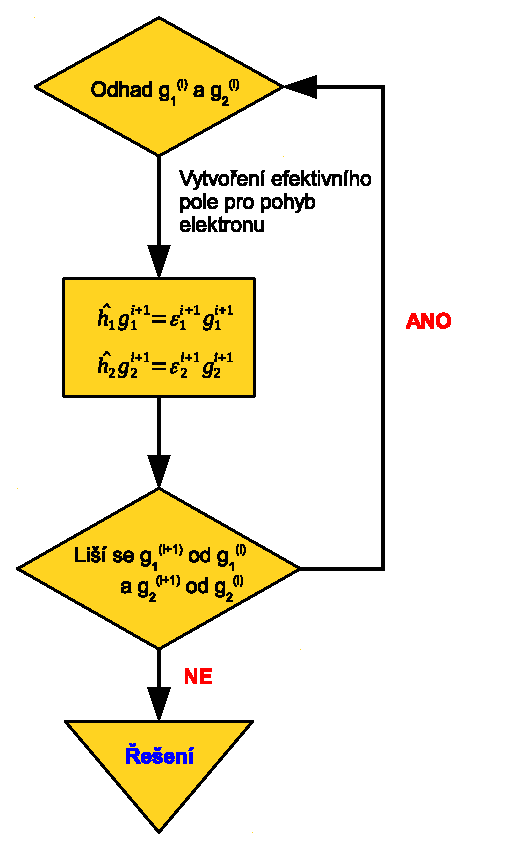
\includegraphics[scale=0.7]{SFCcyklus.eps}
\caption[SCF kolečko]{Řešení Hartreeho a Hartreeho-Fockových rovnice se prakticky provádí iterativním způsobem.}
\label{obr:SCFcycle}
\end{figure}
  
Předvedený postup představuje tzv. Hartreeho metodu. Naše \uv{odvození} bylo heuristické, ke stejnému výsledku bychom ale došli s~použitím variačního počtu. Obecně v~Hartreeho metodě předpokládáme zkusmou vlnovou funkci ve tvaru součinu $N$ jedno-elektronových vlnových funkcí

\begin{equation}
\Phi = q_1 q_2 q_3 \dots q_N.
\label{rov:VE-44}
\end{equation}

\noindent Každý z~elektronů se pak pohybuje v~efektivním potenciálu

\begin{equation}
V_1 (r_1, \theta_1,\phi_1) = \sum_{j=2}^N \frac{e^2}{4 \pi \epsilon_0} \int \frac{\vert q_j \vert^2}{r_{1j}} \mathrm{d}\tau_j - \frac{Z e^2}{4 \pi \epsilon_0 r_1}.
\label{rov:VE-45}
\end{equation}

\noindent Pro každý z~orbitalů $g_i$ pak řešíme jedno-elektronovou Schr\"odingerovu rovnici ve tvaru

\begin{equation}
\hat{h}_i g_i = \varepsilon_i g_i
\label{rov:VE-46}
\end{equation}

Jak vypočítáme celkovou energii? Naivně bychom se mohli domnívat, že stačí sečíst energie jednotlivých elektronů $E = \sum_i \varepsilon_i$. udělali bychom ale chybu, energie $\epsilon_1$ v~sobě zahrnuje coulombovské odpuzování s~druhým až $N$-tým elektronem. Energie interakce mezi prvním a druhým elektronem se ale vyskytuje i ve členu $\epsilon_2$. Mezi-elektronovou repulzi bychom tak započítali dvakráte. Celková energie bude proto dána vztahem

\begin{equation}
E = sum_{i=1}^N \varepsilon_i - \sum_{i=1}^N \sum_{j=i+1}^N \int \int \frac{\vert g_i(i) \vert^2 \vert g_j(j)\vert^2}{4 \pi \epsilon_0 r_{ij}} \mathrm{d}\tau_i \mathrm{d}\tau_j = \sum_{i=1}^N \varepsilon_i - \sum_{i=1}^N \sum_{j=i+1}^N J_{ij},
\label{rov:VE-47}
\end{equation}

\noindent kde druhý člene představuje odpuzování mezi dvěma oblaky elektronů, který odečítáme, aby nebyl započítán dvakrát.


Hartreeho metoda je bohužel pro elektrony nepoužitelná. V~minulé kapitole jsme si vysvětlili, že vlnová funkce popisující elektrony musí být antisymetrická vůči permutaci elektronů. Musíme ji tedy zapsat ve formě Slaterova determinantu

\begin{equation}
\Phi = \frac{1}{N!}
\begin{vmatrix}
g_1(1) \alpha (1) & g_1(2) \alpha (2) & \cdots & g_1(N) \alpha (N) \\
g_2(1) \beta (1) & g_2(2) \beta (2) & \cdots & g_2(N) \beta (N) \\
\vdots & \vdots & \vdots & \vdots \\
g_N(1) \beta (1) & g_N(2) \beta (2) & \cdots &g_N(N) \beta (N)
\end{vmatrix}.
\label{rov:VE-48}
\end{equation}


Tvar jedno-elektronových vlnových funkcí (orbitalů) určíme opět pomocí variační počtu, který nás znovu dovede k~soustavě jedno-elektronových  Schr\"odingerových rovnic, k~tzv. Fockovým rovnicím

\begin{equation}
\hat{F}\phi_i = \varepsilon_i \phi_i,
\label{rov:VE-49}
\end{equation}

\noindent kde se ovšem kromě coulombovských členů vyskytují i tzv. výměnné členy. Mluvíme o~tzv. Hartreeho-Fockových rovnicích. Celkovou energii vypočítáme podobně jako v~Hartreeho metodě

\begin{equation}
E = \sum_{i}^N \varepsilon_i - \sum_{i=1}^N \sum_{j=i+1}^N (J_{ij} - \delta_{ms_i,ms_j} K_{ij}),
\label{rov:VE-50}
\end{equation}

\noindent kde ke coulombovskému integrálu $J_{ij}$ přidanému už v Hartreeho metodě se přidává ještě výměnný integrál


\begin{equation}
K_{ij} = \int \int g_j^{\ast} (\vec{r_1}) g_i^{\ast}(\vec{r_2})) \frac{1}{r_{12}} g_i(\vec{r_1}) g_j(\vec{r_2}) \mathrm{d}\vec{r_1} \mathrm{d}\vec{r_2}.
\label{rov:VE-51}
\end{equation}


\subsection{Roothanovy rovnice}
Jednoelektronové funkce $g_j$ (tedy atomové orbitaly více-elektronových atomů) většinou hledáme ve formě lineární kombinace nějakých známých funkcí $\chi_i$

\begin{equation}
g_j = \sum_i c_{ij} \chi_i.
\label{rov:VE-52}
\end{equation}

\noindent Výhoda je zřejmá, nemusíme hledat neznámé funkce $g_j$, ale pouze neznámá čísla $c_{ji}$. Místo soustavy nelineárních integro-diferenciálních rovnic (Fockových rovnic) řešíme pouze soustavu (nelineárních) algebraických rovnic. Jde o~nám již dobře známé sekulární rovnice

\begin{equation}
\sum_j (F_{ij} - \varepsilon S_{ij}) c_j = 0
\label{rov:VE-53}
\end{equation}

\noindent resp. ve vektorovém zápisu

\begin{equation}
\mathbf{F} \vec{c} = \varepsilon \mathbf{S} \vec{c}.
\label{rov:VE-54}
\end{equation}

Podmínkou netriviálního řešení je nulová hodnota sekulárního determinantu

\begin{equation}
det \vert \mathbf{F} - \varepsilon \mathbf{S} \vert = 0,
\label{rov:VE-55}
\end{equation}

z~čehož dostaneme možné hodnoty energií.

Výše uvedené rovnice se nazývají rovnicemi Roothanovými. 


\subsection{Báze atomových orbitalů}

Množinu funkcí $\chi_i$ nazýváme bází atomových orbitalů.  Tyto funkce mohou být například:
 
\begin{itemize}
\item \textbf{Orbitaly atomů vodíkového typu}. Bohužel tyto funkce jsou pro vyšší hodnoty hlavních kvantových čísel dosti komplikované. Navíc je třeba řada integrálů provádět numericky.

\item \textbf{Orbitaly tzv. Slaterova typu} (STO, z~angl. \textit{Slater Type Orbitals}). Jde o~exponenciální funkce

\begin{equation}
\chi(r) = (2 \xi)^{n+\frac{1}{2}} \left[ (2n)! \right]^{-1/2} r^{n-1} e^{-\xi r}.
\label{rov:VE-56}
\end{equation}

\noindent Na rozdíl od funkcí vodíkového typu nemají STO radiální uzly. Hlavně ale nejsou všechny typy integrálů s~těmito funkcemi analyticky vypočítatelné. 

\item Gaussovské funkce. Tyto funkce mají tvar

\begin{equation}
\chi(r) = N r^n e^{-a(r-r_A)^2}.
\label{rov:VE-57}
\end{equation}

\noindent Nespornou výhodou gaussovských funkcí je skutečnost, že součin dvou gaussiánů je zase gaussián, jenom lokalizovaný na spojnici původních dvou gaussiánů. Všechny maticové elementy jsou analyticky vypočitatelné. Samozřejmě tyto funkce mají i své nevýhody (například nesprávné asymptotické chování), používá se proto lineární kombinace gaussovských funkcí.  

\end{itemize}


Z~praktického hlediska je užitečné seznámit se ještě s~některými pojmy:

\begin{itemize}
\item \textbf{Minimální báze}. V~minimální bázi jsou obsaženy pouze funkce popisující orbitaly obsazené pouze v~základním stavu stavu příslušného atomu. Minimální báze pro atom helia tak obsahuje pouze funkce popisující 1s orbitaly.

\item \textbf{Rozšířená báze}. Tato báze obsahuje funkce jdoucí za rámec minimální báze. Například tzv. polarizační funkce (funkce s~vyšším kvantovým číslem) či funkce difúzní, tj. funkce s~velmi malým exponentem. Tyto funkce jsou důležité kupříkladu pro popis aniontů nebo pro popis slabých mezimolekulárních interakcí. 
 
\end{itemize}

Značení bází atomových orbitalů není nikterak systematické a je zapleveleno historickým vývojem oboru. Z~pohledu uživatele je užitečné mít přehled o~často užívaných zkratkách, jako STO-3G, 6-31g* či aug-cc-pVDZ. Pro detailnější diskusi odkazujeme čtenáře například na Levinovu učebnici kvantové chemie.


\subsection{Periodicita atomů pohledem kvantové teorie}
   
Periodický zákon říká, že vlastnosti prvků jsou periodickou funkcí jeho protonového čísla. Tento zákon byl formulován dlouho před vznikem kvantové mechaniky (a také dlouho před objevením atomového jádra). Kvantová mechanika dává periodickému zákonu novou interpretaci a~na periodickou tabulku nahlíží jako na kvantově-mechanickou strukturu. V~tomto oddíle si kvantově-mechanický pohled na periodicitu vlastností prvků stručně shrneme. 

Zopakujme si nejdříve, jakým způsobem jsou staveny z~elektronů a jader atomy. Základním principům porozumíme v~rámci Hartreeho-Fockovy teorie. Většinou se jako se základními principy setkáme s~následujícími pojmy

\begin{itemize}
\item \textbf{Výstavbový princip}. U~atomů vodíkového typu je energie jedno-elektronového stavu dána výhradně hlavním kvantovým číslem $n$. V~atomech je již degenerace různých stavů se stejným kvantovým číslem sejmuta. Pořadí jednoelektronových stavů, které typicky nalézáme u~neutrálních atomů, nazýváme výstavbovým principem. Podotkněme ovšem, že výstavbový princip není nenarušitelné dogma a pořadí orbitalů je obecně v~různých atomech a~iontech různé, viz obrázek~\ref{obr:Aufbau}.

\begin{figure} [htb]
\centering
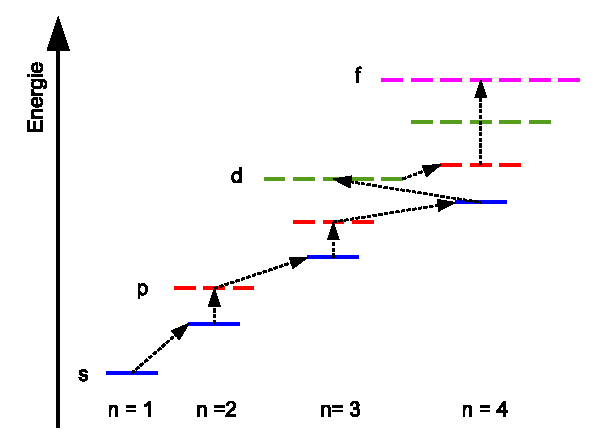
\includegraphics[scale=1]{VystavbovyPrincip.eps}
\caption[Výstavbový princip]{Pořadí orbitalů, které typicky nacházíme v~neutrálních atomech, se nazývá výstavbovým principem.}
\label{obr:Aufbau}
\end{figure}

\item \textbf{Pauliho vylučovací princip}. Zcela fundamentální princip, bez něj by periodická tabulka neexistovala, všechny prvky by v~základním stavu byly jenom různě vypasené atomy vodíku.

\item \textbf{Pravidlo maximální multiplicity}. O~Hundových pravidlech bude řečeno více dále.   
 
\end{itemize}

\noindent Z~Fockových rovnic také vyplývá tzv. Koopmansův teorém, dle kterého ionizační energie i-tého elektronu $IE_i$ rovna orbitální energii příslušného elektronu $\epsilon_i$ (až na znaménko) 

\begin{equation}
IE_i = - \varepsilon_i
\label{rov:VE-58}
\end{equation}

\noindent a orbitální energie nejnižšího neobsazeného elektronu (LUMO elektronu, z~angl. \textit{Lowest Unoccupied Molecular Orbital}) je zase rovna elektronové afinitě

\begin{equation}
EA = -\varepsilon_{\mathrm{LUMO}}.
\label{rov:VE-59}
\end{equation}

Pojďme se nyní podívat, jak se vyvíjí s~protonovým číslem kupříkladu ionizační energie nejvýše obsazeného elektronu (HOMO elektronu, z~angl. \textit{Highest Occupied Molecular Orbital}). Pro atom vodíkového typu by platilo

\begin{equation}
IE \sim \frac{(Z^{\prime})^2}{n^2}.
\label{rov:VE-60}
\end{equation}

\noindent Vnitřní elektrony ale velmi efektivně stíní náboj jádra, takže HOMO elektron cítí náboj zmenšený o~počet elektronů ve vnitřních slupkách. Jestliže se budeme pohybovat v~periodě od lithia k~neonu, očekávali bychom rostoucí ionizační energii: roste totiž protonové číslo a náboj jádra není ještě stíněn. Jestliže ale od neonu přejdeme k~sodíku, vzroste najednou skokově hlavní kvantové číslo $n$ a navíc efektivní protonové číslo se zmenší díky stínění náboje jádra vnitřními elektrony. Ionizační energie by se proto měla spíše blížit lithiu nežli neonu. To skutečně pozorujeme (pohleď, čtenáři, na obrázek~\ref{obr:Period}). Podobné úvahy vysvětlí i periodické změny poloměru atomů, který je pro jedno-elektronové atomy dán vztahem

\begin{equation}
R \sim \frac{n^2}{Z^{\prime}},
\label{rov:VE-61}
\end{equation}

\noindent či třeba periodicita elektronegativity, kterou můžeme dle Mullikena definovat jako

\begin{equation}
\chi = 0{,}187 (IE + EA) + 0{,}17.
\label{rov:VE-62}
\end{equation}

\begin{figure} [htb]
\centering
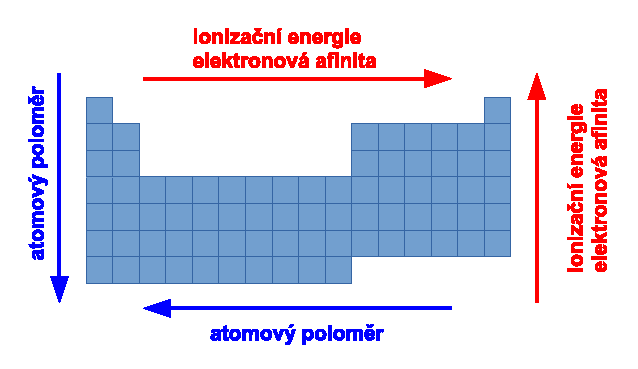
\includegraphics[scale=1]{PeriodicitaVlastnosti.eps}
\caption[Periodicita vlastností prvků]{Ionizační energie, elektronové afinity či poloměry atomů se s~protonovým číslem periodicky mění. Tato periodicita je důsledkem základních kvantově-mechanických zákonů.}
\label{obr:Period}
\end{figure}


\subsection{Sčítání momentu hybnosti a atomové termy}
Jedno-elektronové atomy jsou charakterizovány nejen energií, ale také hodnotou velikosti momentu hybnosti (kvantové číslo $l$) a projekcí momentu hybnosti do určité osy (konvenčně do osy z, kvantové číslo $m$). Jestliže studujeme atomy s~více elektrony, mohlo a mělo by nás zajímat, jakým způsobem se momenty hybností jednotlivých elektronů sčítají do celkového momentu hybnosti.

Celkový moment hybnosti $\vec{L}$ by měl splňovat kvantově-mechanická pravidla jako jakýkoliv jiný moment hybnosti. Pro jeho velikost tak bude platit

\begin{equation}
\vert \vec{L} \vert = \hbar \sqrt{L(L+1)}
\label{rov:VE-63}
\end{equation}

\noindent a pro projekci do směru osy $z$ pak

\begin{equation}
L_z = \hbar M.
\label{rov:VE-64}
\end{equation}
 

Uvažme případ dvou elektronů, z~nichž každý se nachází v~p orbitalu a je tedy charakterizován kvantovým číslem $l=1$.

\begin{eqnarray*}
l_1 &=& 1 \\
l_2 &=& 1
\end{eqnarray*}

\noindent Hodnota momentu hybnosti ve směru osy $z$ se pak může buďto sčítat a nebo odčítat. Udělejme si následující tabulku

\begin{table}[ht]
\centering
\begin{tabular}{c|ccc}
\toprule
    $_{m_1}\ddots^{m_2}$      & -1    & 0     & 1 \\
\midrule
    -1    & -2    & -1    & 0 \\
    0     & -1    & 0     & 1 \\
    1     & 0     & 1     & 2 \\
\bottomrule
\end{tabular}
\label{tab:ScitaniHybnosti}
\end{table}



Vidíme, že bude existovat stav, pro který kvantové číslo $M$ určující projekci celkového momentu hybnosti do osy $z$ nabývá hodnoty 2. Tomu ale odpovídá stav s~velikostí momentu hybnosti daného kvantovým číslem $L = 2$. K~tomuto kvantovému číslu ovšem přísluší ještě hodnoty $M=+1,0,-1,-2$. V~tabulce nám tedy zbývají hodnoty $M =-1,0,0,1$. Je zjevné, že tedy musí existovat i stav s~hodnotou $L=1$. Tomu odpovídají hodnoty $M=-1,0, 1$. Zbývá tedy ještě $M=0$, čemuž odpovídá $L=0$. Vidíme tedy, že ze dvou elektronů ve stavu $l=1$ můžeme dostat $L=2,1,0$. 

Tuto naši úvahu můžeme zobecnit. Máme-li dva elektrony ve stavu $l_1$ a $l_1$, pak celkový moment hybnosti může nabývat hodnot

\begin{equation}
L = \vert l_1 - l_2 \vert , \dots , l_1 + l_2.
\label{rov:VE-65}
\end{equation}

Stejným způsobem můžeme sčítat také celkový orbitální moment $\vec{L}$ a celkový spinový moment $\vec{S}$ do celkového momentu $\vec{J} = \vec{L} + \vec{S}$. Pro kvantové číslo $J$ bude platit

\begin{equation}
J = \vert L - S \vert, \dots, L+S.
\label{rov:VE-66}
\end{equation}


Stav atomu potom zapisujeme pomocí tzv. atomového termu


\begin{figure} [ht]
\centering
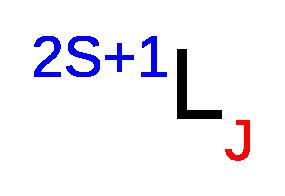
\includegraphics[scale=0.8]{AtomovyTerm.eps}
\caption[Atomové termy]{Symbol používaný pro vyjádření stavu mnoho-elektronového atomu}
\label{obr:ATerm}
\end{figure}

\begin{priklad}
\textbf{Zadání:} Při plamenných zkouškách je nejsnadnější poznat přítomnost sodíku díky vyzařování intenzivního žlutého světla. Toto světlo odpovídá přechodu nepárového elektronu z 2p orbitalu sodíku do orbitalu 2s. Už v 19. století se zjistilo, že jde o~dvě velmi blízko ležící čáry,  jedna u 589,0~nm a druhá u 589,6~nm. Jakým dvěma přechodům tyto emisní čáry odpovídají?\\[0.1cm]
\textbf{Řešení:} Sodík s nepárovým  elektronem v 2p orbitalu se může nacházet ve dvou stavech lišícím se kvantovým číslem J. Kvantové číslo $L=1$, kvantové číslo $S=1/2$, pak $J=|L-S|,\, L+S$ tedy dá $J=1/2,\,3/2$.

Půjde tedy o přechody ze stavů $^2$P$_{1/2}$ a $^2$P$_{3/2}$ do $^2$S$_0$ stavu, což je základní stav atomu sodíku. Dle Hundových pravidel bude energeticky níže stav $^2$P$_{1/2}$, tj. přechod u 589,6~nm odpovídá deexcitaci z tohoto stavu.
\end{priklad}

Musíme mít ovšem na paměti, že ne všechny součty jsou v~atomech možné (díky Pauliho vylučovacímu principu).



\subsubsection{Hundova pravidla}
Pořadí jednotlivých atomových termů dle energie je dáno tzv. Hundovými pravidly. Níže uvádíme jejich přehled.

\begin{itemize}
\item Term s~maximální multiplicitou má nejnižší energii.

\item Je-li multiplicita dvou termů stejná, pak nižší energii má term s~vyšší hodnotou $L$.

\item Je-li multiplicita i $L$ dvou termů stejná, pak pro slupky méně než z~poloviny zaplněné má nižší energii stav s~nižším $J$.  
 
\end{itemize}

\begin{priklad}
\textbf{Zadání:} S pomocí Hundových pravidel odvoďte základní stav atomu uhlíku a~zapište dovolené termy.\\[0.1cm]
\textbf{Řešení:} Základní elektronový stav má plnou elektronovou konfiguraci
\begin{displaymath}
1\mathrm{s}^2 \, 2\mathrm{s}^2 \, 2\mathrm{p}^2
\end{displaymath}
nebo ve zkrácené podobě
\begin{displaymath}
^{2} \mathrm{He}: 2\mathrm{s}^2 \, 2\mathrm{p}^2.
\end{displaymath}
Dále víme, že plně zaplněné slupky nemusíme uvažovat. Došli jsme tak k~závěru, že základní stav atomu uhlíku odpovídá elektronové konfiguraci 2p$^2$. Tomu odpovídají termy
\begin{displaymath}
^{1}\mathrm{S}_0, \, ^{3}\mathrm{P}_0, \, ^{3}\mathrm{P}_1, \, ^{3}\mathrm{P}_2 \mbox{ a } ^{1}\mathrm{D}_2.
\end{displaymath} \vspace{-0.7cm}
\end{priklad}


V~nerelativistické kvantové mechanice by se energie stavů lišících se pouze hodnotou celkového momentu hybnosti $J$ neměla lišit. Rozdíl energií je způsoben tzv. spin-orbitální vazbou. Zhruba řečeno, elektron rotující kolem jádra generuje magnetické pole. Spin elektronu je vůči tomuto poli různým způsobem orientován a tím je ovlivněna i jeho energie. V~hamiltoniánu tak přibývá člen

\begin{equation}
\hat{H}_{SO} = \xi \hat{L} \hat{S}.
\label{rov:VE-67}
\end{equation}

\noindent Parametr $\xi$ představuje pro lehká jádra jenom velmi malý člen, Ten však rychle roste a pro těžká jádra je třeba tento jev brát v~potaz. Sčítání momentů hybnosti se dá provádět dvojím způsobem

\begin{itemize}
\item \textbf{L-S vazba (Russelova-Saundersova)}. Zde nejdříve sčítáme orbitální moment hybnosti pro celý atom, zvláště spinový moment pro celý atom a teprve na konci sečteme oba momenty. Uplatňuje se v~situacích, kdy je mezi-elektronová repulze významnějším efektem v~porovnání se spin-orbitální vazbou.  

\item \textbf{j-j vazba}. Zde nejdříve sčítáme orbitální a spinový moment pro jednotlivé elektrony a~sčítáme teprve výsledný moment hybnosti. 

\end{itemize}     



   
    


   

 



 




 
